\section{ارتباط بین دو آردوینو با استفاده از پروتکل \lr{SPI}}

\subsection{اهداف آزمایش}
\begin{itemize}
    \item آشنایی با پروتکل ارتباطی \lr{SPI}
    \item آشنایی با پروتکل سریال و ارتباط با کامپیوتر از طریق آن
\end{itemize}

\subsection{قطعات مورد نیاز}
\begin{itemize}
    \item \lr{Arduino Uno}
\end{itemize}

\subsection{مقدمه}
تا اینجا آردوینوی ما ارتباطی با کامپیوتری که از طریق آن برنامه ها را روی آن آپلود می‌کردیم نداشت. می‌توانیم با استفاده از ارتباط سریال، این کار را انجام دهیم. برای این کار کافیست از کتاب‌خانه‌ی سریال استفاده کنیم.
\newline
\textcolor{red}{\begin{nas}سوال: \end{nas}}
در مستندات آردوینو جست‌و‌جو کنید و در مورد توابع کتاب‌خانه‌ی \lr{Serial} توضیح دهید.
\newline
با پروتکل \lr{SPI} در درس ریزپردازنده آشنا شدید.
همانطور که می‌دانید این نوع ارتباط از نوع ارتباطات \lr{Master\Slave} است. در این نوع ارتباطات یک دستگاه می‌تواند با چند دستگاه دیگر ارتباط برقرار کند. در ارتباط \lr{SPI} بورد مرکزی یا همان \lr{Master} بوردی که میخواهد با آن ارتباط برقرار کند را انتخاب کرده و برای آن پیامی ارسال می‌کند و در صورت نیاز، از آن درخواست پاسخ می‌کند.
\newline
\textcolor{red}{\begin{nas}سوال: \end{nas}}
در مورد پروتکل \lr{SPI} به سوالات یر پاسخ دهید:
\begin{itemize}
    \item این پروتوکل از ۴ سیم استفاده می‌کند. وظیفه‌ی هر یک از این ۴ سیم را شرح دهید.
    \item آیا این پروتکل امکان حضور چند \lr{Master} را به ما می‌دهد؟
    \item در بورد \lr{Arduino Uno} کدام پین های به صورت پیش‌فرض برای پین های \lr{SPI} تخصیص داده شده‌اند؟
    \item در این پروتکل ارتباطی سنکرون، کلاک توسط \lr{Master} تعیین می‌شود یا \lr{Slave}؟
\end{itemize}
\newline
می‌توانیم برای استفاده از این پروتکل، از کتابخانه‌ی \lr{SPI.h} استفاده کنیم. این کتاب‌خانه یک لایه‌ی انتزاع برای ارتباط با سخت‌افزار مخصوص \lr{SPI} در میکروکنترلر های مختلف است و این اجازه را به ما می‌دهد که به صورت نسبتا \lr{Portable} برنامه‌ای بنویسیم که از این کتاب‌خانه استفاده کند.
\newline
\textcolor{red}{\begin{nas}سوال: \end{nas}}
در مستندات این کتاب‌خانه جستوجو کنید و در مورد توابع زیر توضیح بدهید:
\begin{itemize}
    \item \lr{SPI.begin()}
    \item \lr{SPI.beginTransaction()}
    \item \lr{SPI.end()}
    \item \lr{SPI.transfer()}
    \item \lr{SPI.usingInterrupt()}
\end{itemize}
در این آزمایش باید آردوینوی ما هم در حالت \lr{Master} و هم در حالت \lr{Slave} کار کند.
\newline
\textcolor{red}{\begin{nas}سوال: \end{nas}}
دستوری که با استفاده از آن آردوینو در حالت \lr{Slave} قرار می‌گیرد را بنویسید و آن را توضیح دهید.

\subsection{شرح آزمایش}

می‌خواهیم یک پیام را از یک آردوینو به آردوینو دیگر انتقال دهیم و برای این کار از پروتکل \lr{SPI} استفاده می‌کنیم.
هر یک از گروه ها باید برنامه \lr{Master} و \lr{Slave} خود را درست کنند و با برنامه متناظر گروه دیگر آزمایش کنند.
\newline
برنامه \lr{Master} باید با استفاده از پروتکل \lr{Serial} یک متن را از ورودی بگیرد و با استفاده از \lr{SPI} آن را به برنامه‌ی \lr{Slave} بدهد. برنامه‌ی \lr{Slave} نیز باید پیام را دریافت کرده و از طریق پروتکل \lr{Serial} نمایش بدهد.

\newline

توجه داشته باشید که دستگاه \lr{Slave} حتما باید در حالت \lr{Slave} قرار بگیرند. در غیر این صورت هر دو دستگاه می‌خواهند کلاک را خودشان تامین کنند و احتمال خرابی قطعات وجود دارد. می‌توانید برای اطلاعات بیشتر به
\href{https://circuitdigest.com/microcontroller-projects/arduino-spi-communication-tutorial}{این لینک}
مراجعه کنید.

\newline
\begin{figure}[h]
    \centering
    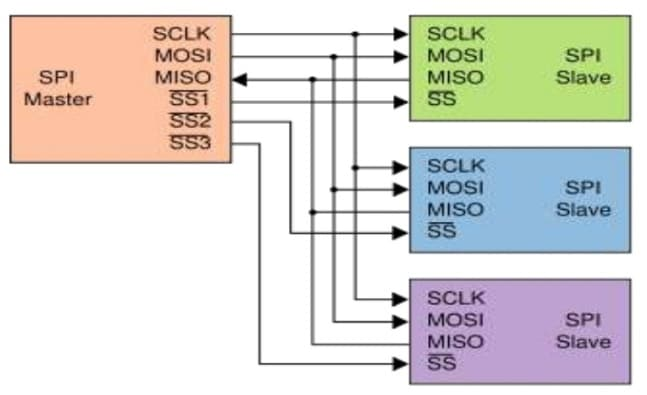
\includegraphics[width=8cm]{SPI_BUS.jpg}
    \caption{یک نمونه از باس \lr{SPI}}
    \label{fig:spibus}
\end{figure}
\newline

توجه کنید که در شکل پین‌های بورد آردوینو که در بخش مقدمه‌ی دستور کار آمده به جای اسامی \lr{MISO} و \lr{MOSI} به ترتیب از \lr{CIPO} و \lr{COPI} استفاده شده است.